\documentclass[aps,preprint,nofootinbib,floatfix]{revtex4-1}

%\usepackage{cite}
\usepackage[pdftex]{graphicx}
\graphicspath{{./figures/}}
%\graphicspath{{./}}
\usepackage{amsmath,amssymb,amsfonts,amsthm,amscd,bm}
\usepackage{bbm}
\usepackage{algorithm}
\usepackage{algorithmic}
%\usepackage{epstopdf}
%\usepackage{fixltx2e}
%\usepackage{stfloats}

\hyphenation{op-tical net-works semi-conduc-tor}

\newtheorem{theorem}{Theorem}
\newtheorem{definition}[theorem]{Definition}
\newtheorem{assumption}[theorem]{Assumption}
\newtheorem{lemma}[theorem]{Lemma}
\newtheorem{corollary}[theorem]{Corollary}
\newtheorem{proposition}[theorem]{Proposition}
\newtheorem{conjecture}[theorem]{Conjecture}
\newtheorem{remark}[theorem]{Remark}
\newtheorem{example}{Example}

%% our definitions %%%%%%%%%%%%%%%%%%%%%%%%%%%%%%%%%%%%%%%%%%%%%%%%%%%%%%%%%%%%
\DeclareMathOperator{\aff}{aff}
\DeclareMathOperator{\st}{s.t.}
\DeclareMathOperator{\LC}{LC}
\DeclareMathOperator{\affnot}{aff_0}
\DeclareMathOperator{\conv}{conv}
\DeclareMathOperator{\relint}{relint}
\DeclareMathOperator{\vol}{vol}
\DeclareMathOperator{\range}{range}
\DeclareMathOperator{\image}{im}
\DeclareMathOperator{\nullspace}{null}
\DeclareMathOperator{\area}{area}
\DeclareMathOperator{\vspan}{span}
\DeclareMathOperator{\id}{Id}
\DeclareMathOperator{\cond}{cond}
\DeclareMathOperator{\prox}{prox}
\DeclareMathOperator*{\argmax}{arg\,max}
\DeclareMathOperator*{\argmin}{arg\,min}
\DeclareMathOperator*{\minimize}{minimize}
\DeclareMathOperator{\diag}{diag}
\DeclareMathOperator{\Tr}{Tr}

\graphicspath{{figs/}}

\begin{document}

\title{Discussion about $k$-Means and $1D$ Random Projections}

\author{Guilherme Fran\c ca}
%\email{guifranca@gmail.com}
%\affiliation{Johns Hopkins University, Center for Imaging Science}

\maketitle

\section{Procedure}

Given data $X=\{ x_i \}_{i=1}^{n}$, where $x_i \in \mathbb{R}^{D}$, 
and the number of clusters $k$, we perform the following experiments:
\begin{enumerate}
\item Run $k$-means$++$ 
on the original data. This is the column named 
``$k$-means'' in the following tables.
\item Use PCA to 
project the data in the first principal component, 
$Y=\{ y_i \}_{i=1}^n$ where $y_i = u_{1}\cdot x_i \in \mathbb{R}$, then
apply $k$-means in this $1$-dimensional space. This is the column named
``PCA'' in the following tables.
\item We randomly project the data in one dimension by picking a vector
$w$ such that $w_i \sim \mathcal{N}(0,1)$ and normalize it $\| w \|=1$.
Thus $Y = \{y_i\}_{i=1}^n $ where $y_i = w\cdot x_i \in \mathbb{R}$. 
We apply $k$-means in this randomly projected
$1$-dimensional space. We do this several times and pick the best answer.
This is the column named ``$k$-random'' in the following tables.
We will choose 100 random projections.
\item We use random projections as in the previous item, but use the $T$-test
from energy statistics. In $1D$ we can compute the energy distance in an
efficient manner if we sort the data $Y$. This is the column called
``$\mathcal{E}$-random'' in the following tables.
We will choose 100 random projections.
\end{enumerate}

The evaluation of the clustering procedure 
will be based on the true labels by the following quantity, called
accuracy:
\begin{equation}
\label{eq:accuracy}
a(z,\hat{z}) = 
\dfrac{1}{n}\sum_{i=1}^{n} \mathbbm{1}\left(z_i = \pi(\hat{z}_i) \right)
\end{equation}
where $z$ is an $n$-dimensional vector containing the true labels, entry
$z_i$ corresponds to point $x_i$, and $\hat{z}$ is the estimated labels
through the clustering procedure. $\pi$ is a permutation of the labels.
Thus the above formula gives $a=1$ if all points were correctly classified and
$a=0$ if all points were wrongly classified. In a two class problem with
the same number of points, $a=1/2$ corresponds to picking the points in each
cluster at random. 
This quantity $a$ is the number shown in the following tables.


\paragraph*{How to choose the best answer for random projections?}
In the following experiments we are going to cheat and pick the best answer
according to the highest value of \eqref{eq:accuracy}. This is cheating because
we are using the true labels, however, this test allows us to easily
check if the ``truth'' can be captured by these procedures involving
random projections. If the results
are poor in this way, no matter what criteria we choose, optimizing 
$\mathcal{E}$ or any other function will also not work.

\paragraph*{Note:} The procedures involving random projections are much
slower than simple $k$-means in the original data. It is also much slower
than PCA$+$$k$-means. Moreover, computing random projections in high
dimensions is also a little expensive. Doing this many times can make
the algorithm really slow.

%Consider $k$-means objective function
%\begin{equation}
%\label{eq:J}
%J(X) = \dfrac{1}{2} \sum_{j=1}^k \sum_{x \in \mathcal{C}_j} \| x - m_j \|^2,
%\qquad
%m_j = \dfrac{1}{n_j}\sum_{x\in\mathcal{C}_j} x.
%\end{equation}
%Above $m_j$ is the center
%of cluster $\mathcal{C}_j$, and 
%$n_j$ is the number of elements in cluster $\mathcal{C}_j$. $k$-means
%algorithm solves the problem $\min_{\{C_j\}} J(X)$. 
%
%One might think
%that a good criteria to choose the best answer is to pick the minimum $J(Y)$
%computed in the $1D$ randomly projected space. This doesn't work because
%each random projection gives different values for the data $Y$ which in general
%does not preserve the structure in the original
%distribution. For instance, considering two random projections yielding
%$Y_1$ and $Y_2$. It can happen that the clustering on $Y_2$ gives a better
%accuracy than the clustering on $Y_1$ and even though $J(Y_1) < J(Y_2)$.
%So we are really comparing apples and bananas here.
%
%Another approach would be to cluster on $Y$ yielding labels $\hat{z}$, then
%compute $J(X)$ based on these labels, and pick the smallest $J(X)$  computed
%on the original data. This only works in case where $k$-means in the original
%space itself provides a good answer. For cases where $k$-means is problematic,
%e.g. the data are not spherical gaussians, then $J(X)$ itself is not a good
%function to detect the clustering. This happens for parallel cigars in the
%example below.
%
%Thus if one still desires to follow this approach, a good function which
%does not depend on the true labels must be chosen. I tried to use the energy
%function for this, and still didn't quite work. Also, observe that the 
%energy function on the original space is expensive to compute, 
%$O(n^2)$.
%
%In the following experiments I will \emph{cheat} and use \eqref{eq:accuracy}
%to pick the best answer. The purpose of this is to see if the ``truth'' can
%be captured by random projections.

\section{First Experiments}

In the first experiment shown in Fig.~\ref{fig:2d_gauss_sep} we choose
two well separated gaussians in $2D$. All of these procedures give good
results.

\begin{figure}
\begin{minipage}{.49\textwidth}
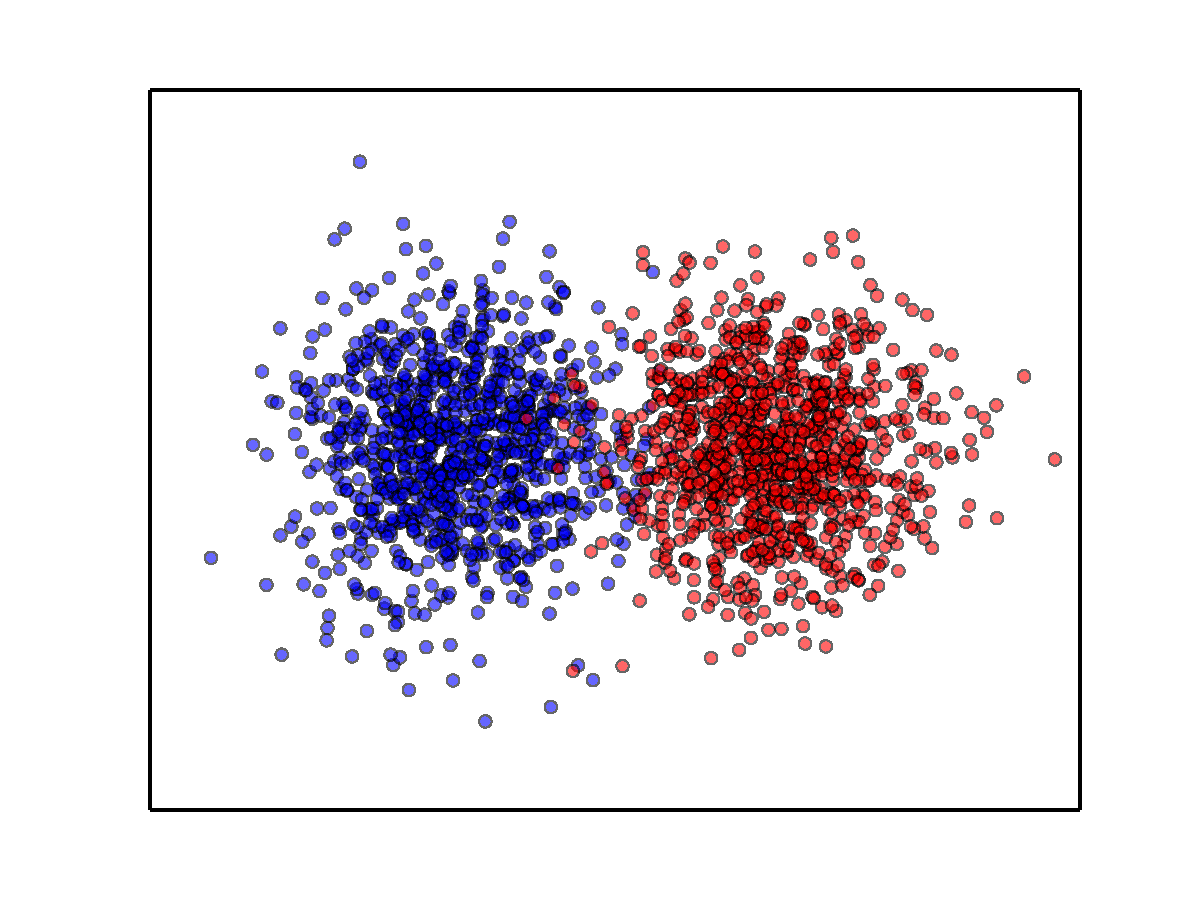
\includegraphics[scale=.45]{2d_gauss_separate.pdf}
\end{minipage}
\begin{minipage}{.49\textwidth}
\begin{tabular}{ l  l  l l}
\hline
$k$-means~ & PCA~~~ & $k$-random~ & $\mathcal{E}$-random \\
\hline
0.9735 &
0.9735 &
0.9745 &
0.976 \\
%
0.9745 &
0.975 &
0.976 &
0.975 \\
%
0.973 &
0.9735 & 
0.976 &
0.976 \\
%
\hline
\end{tabular}
\end{minipage}
\caption{\label{fig:2d_gauss_sep}
We have $x \sim \tfrac{1}{2}\left( \mathcal{N}(\mu_1, I) +
\mathcal{N}(\mu_2, I)\right)$ where $\mu_1 = (0,0)^T$ and $\mu_2=(4,0)^T$,
and $1000$ points on each cluster. We run the experiment three times.
}
\end{figure}

In the experiment of Fig.~\ref{fig:cigar}, still in $2D$, we choose
parallel cigars. Both $k$-means and PCA cannot perform well, however random
projections can do well. This is not surprising because this data
can be linearly separable in $1D$. After many tries random projections will
find the correct line. Probably, LDA can perform as well on this example.

\begin{figure}
\begin{minipage}{.49\textwidth}
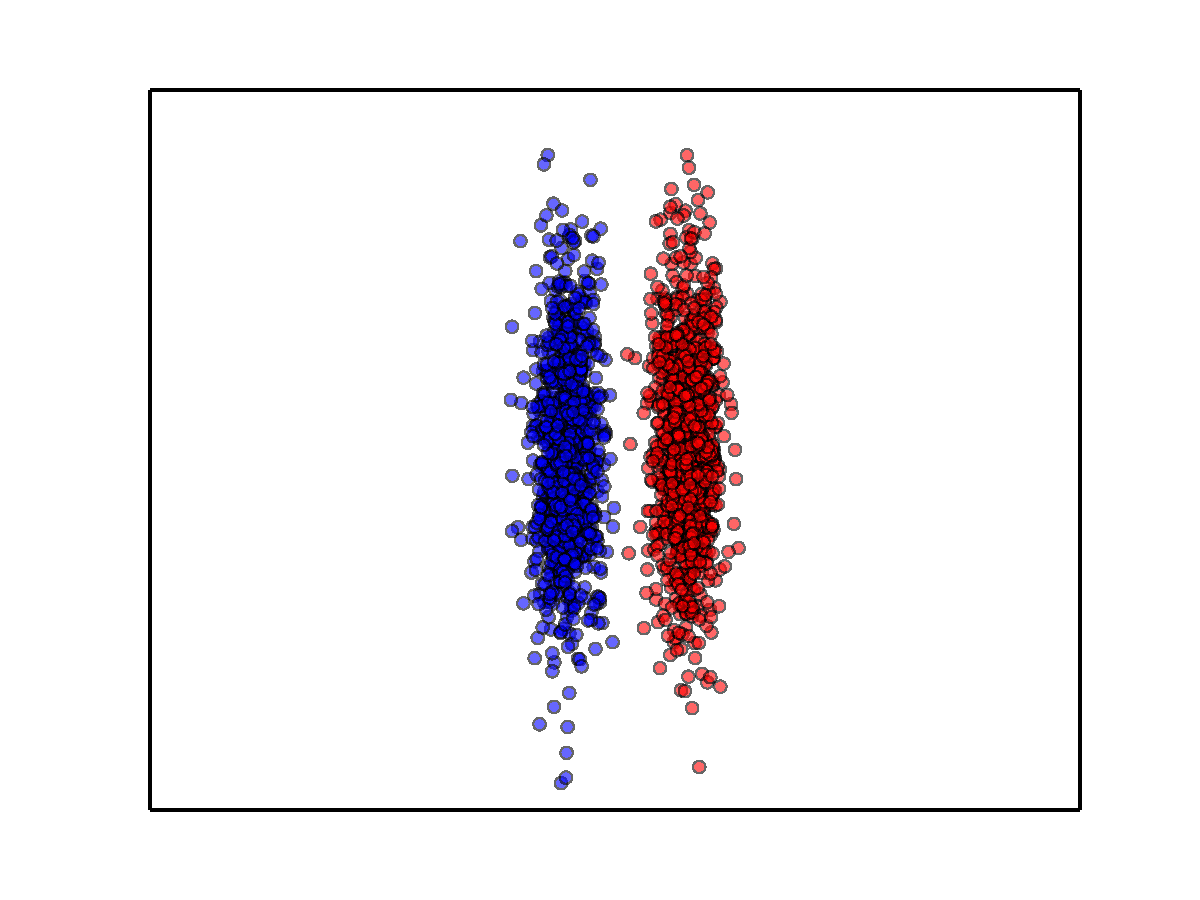
\includegraphics[scale=.45]{2d_cigar.pdf}
\end{minipage}
\begin{minipage}{.49\textwidth}
\begin{tabular}{ l l l l}
\hline
$k$-means~ & PCA~~~ & $k$-random~ & $\mathcal{E}$-random \\
\hline
0.5085 &
0.5025 &
1.0 &
1.0 \\
%
0.5025 &
0.5035 &
1.0 &
1.0 \\
%
0.503 &
0.5 &
1.0 &
1.0 \\
%
\hline
\end{tabular}
\end{minipage}
\caption{\label{fig:cigar}
We have $x \sim \tfrac{1}{2}\left( \mathcal{N}(\mu_1, \Sigma) +
\mathcal{N}(\mu_2, \Sigma)\right)$ where $\mu_1 = (0,0)^T$, $\mu_2=(5,0)^T$,
and $\Sigma = \left( \begin{smallmatrix} 1/2 & 0 \\ 0 & 15 \end{smallmatrix}
\right)$,
and $1000$ points on each cluster. We run the experiment three times.
}
\end{figure}

In the experiment of Fig.~\ref{fig:weird1} notice that the $k$-means with
random projections performs better than any other method.

\begin{figure}
\begin{minipage}{.49\textwidth}
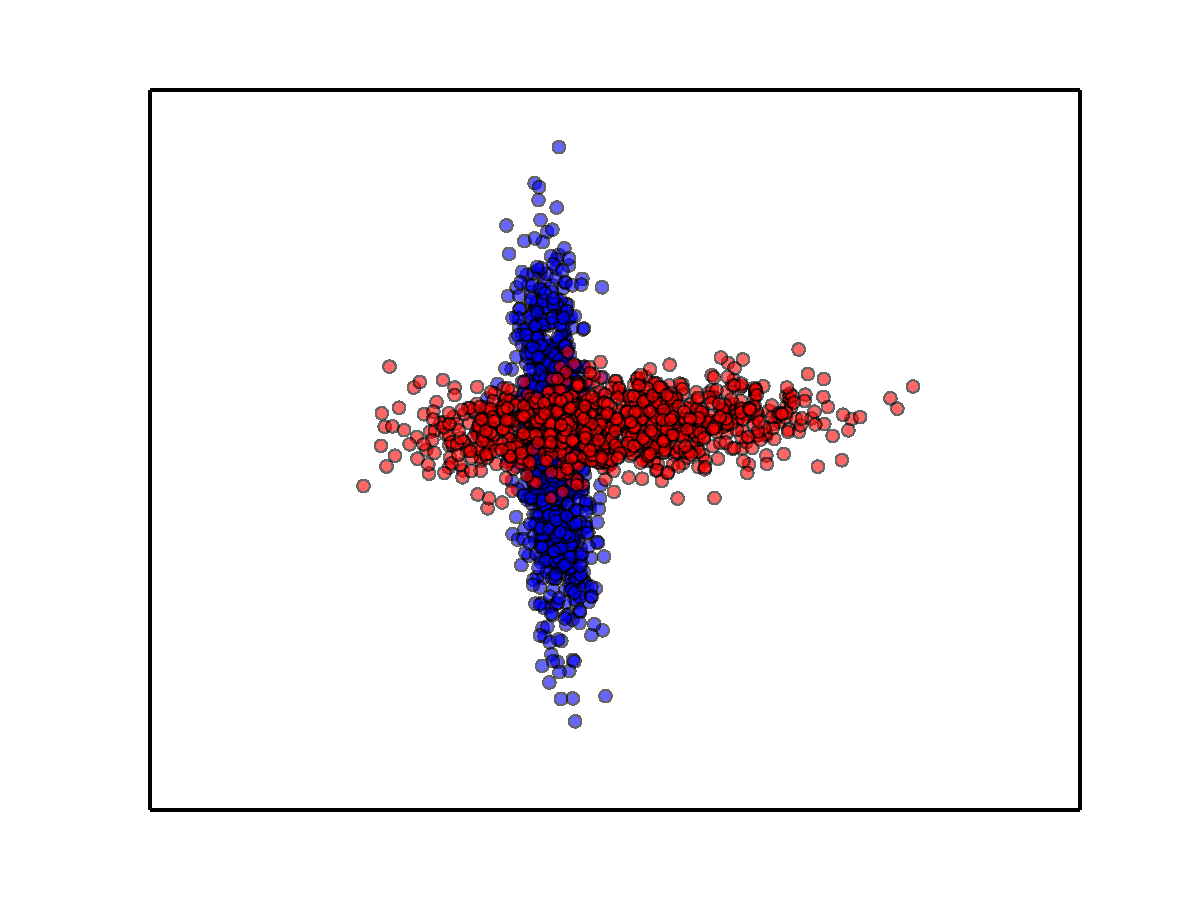
\includegraphics[scale=.45]{2d_weird1.pdf}
\end{minipage}
\begin{minipage}{.49\textwidth}
\begin{tabular}{ l l l l}
\hline
$k$-means~ & PCA~~~ & $k$-random~ & $\mathcal{E}$-random \\
\hline
0.6315 &
0.6295 &
0.7235 & 
0.66 \\
%
0.725 &
0.7065 &
0.726 &
0.678 \\
%
0.6405 &
0.6465 &
0.724 & 
0.679 \\
%
\hline
\end{tabular}
\end{minipage}
\caption{\label{fig:weird1}
We have $x \sim \tfrac{1}{2}\left( \mathcal{N}(\mu_1, \Sigma_1) +
\mathcal{N}(\mu_2, \Sigma_2)\right)$ where $\mu_1 = (0,0)^T$, $\mu_2=(2,1)^T$,
$\Sigma_1 = \left( \begin{smallmatrix} 0.5 & -0.8 \\ -0.8 & 15 
\end{smallmatrix}
\right)$,
$\Sigma_2 = \left( \begin{smallmatrix} 15 & 1 \\ 1 & 1 \end{smallmatrix}
\right)$,
and $1000$ points on each cluster. We run the experiment three times.
}
\end{figure}


In the experiment of Fig.~\ref{fig:highd} we increase the number of
dimensions of the gaussian distributions. Both $k$-means and PCA perform well
if the dimension is not too high, while $1D$ random projections provide
poor results. This is also expected since randomly projecting high dimensional
data in a very low dimensional space practically destroy any information
about the original distribution.

\begin{figure}
\begin{minipage}{.49\textwidth}
\centering
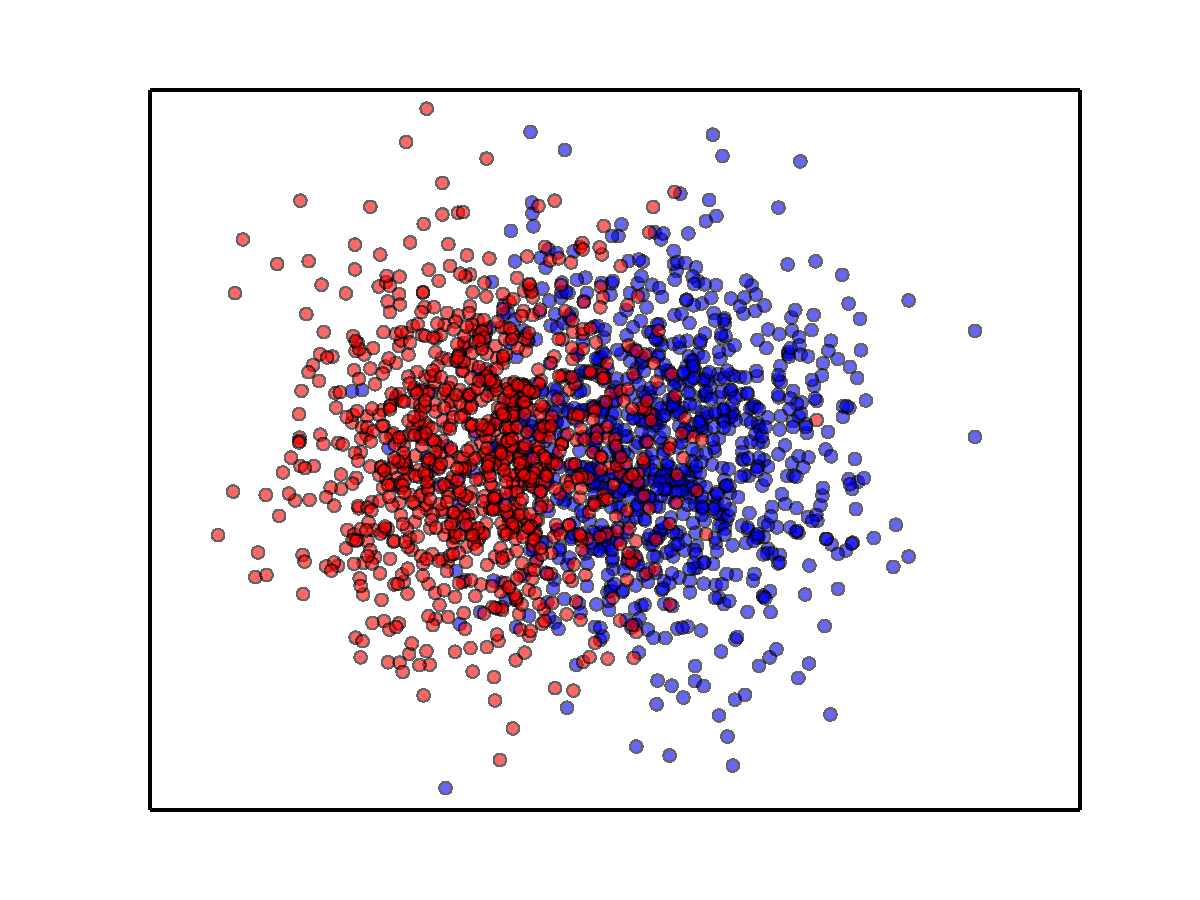
\includegraphics[scale=.45]{30d_gauss.pdf}
\end{minipage}
\begin{minipage}{.5\textwidth}
\renewcommand*{\arraystretch}{.3}
\begin{tabular}{l l l l l}
\hline
$D$ & $k$-means & PCA & $k$-random & $\mathcal{E}$-random \\
\hline
%
5 & 0.934500 & 0.934500 & 0.919000 & 0.924000 \\
10 & 0.939500 & 0.941500 & 0.912000 & 0.856000 \\
15 & 0.933000 & 0.935000 & 0.882000 & 0.816000 \\
20 & 0.940000 & 0.942000 & 0.762000 & 0.817000 \\
25 & 0.931500 & 0.933500 & 0.767000 & 0.759000 \\
30 & 0.936000 & 0.934000 & 0.754000 & 0.725000 \\
50 & 0.946000 & 0.942500 & 0.718500 & 0.741000 \\
100 & 0.926500 & 0.927000 & 0.658500 & 0.647000 \\
200 & 0.940000 & 0.940000 & 0.604000 & 0.647000 \\
300 & 0.918000 & 0.921500 & 0.592500 & 0.602000 \\
500 & 0.915000 & 0.922000 & 0.596500 & 0.576000 \\
1000 & 0.874000 & 0.890500 & 0.552000 & 0.574000 \\
2000 & 0.597000 & 0.863500 & 0.542000 & 0.554000 \\
5000 & 0.509000 & 0.788000 & 0.543000 & 0.540000 \\
%
\hline
\end{tabular}
\end{minipage}
\caption{\label{fig:highd}
High dimensions.
We have $x \sim \tfrac{1}{2}\left( \mathcal{N}(\mu_1, I_D) +
\mathcal{N}(\mu_2, I_D)\right)$ where $\mu_1 = (0,0,\dotsc,0)^T$,
$\mu_2=(3,0,\dots,0)^T$,
and $1000$ points on each cluster. We show the two principal components
of the data in the plot above.
}
\end{figure}


\section{Second Experiments}

We repeated the experiments above using the objective function as a criteria
instead of the accuracy \eqref{eq:accuracy} so we do not use the true labels.
We computed the objective function in the $1D$ projected space. 

For $k$-means
the function is the sum of squared distances from the points 
to the centers of the clusters,
and for energy statistics we compute the ``energy'' $\mathcal{E}$ in the
$1D$ space, which can be done in $O(n \log n)$. The results are just slightly
worse than before because not always the optimal function coincides with
the best clustering. Notice that we are comparing these functions on 
different data sets, one for each projection. Thus this is not a very
consistent way of doing the test.


\section{Conclusions}

These are just my thoughts about why random projections in $1D$ 
does not work
for \emph{clustering}---it surely
must work with random projections in higher dimensions though, since
we have Johnson-Lindenstrauss lemma that guarantees that distances
are preserved in lower dimensional spaces, but they are not so 
low-dimensional---regardless of 
the function you are trying to optimize,
e.g. $k$-means objective function, energy statistics, whatever, etc.

In $1D$, random projections just seems to me a more expensive way of doing
LDA. In $1D$ the best line which separates the data (I believe) is the line
passing through the means of each cluster (I'm thinking about two clusters
only). If data is not linearly separable
in $1D$, neither of both methods work.

Although $\mathcal{E}$ seems a nice function, which can distinguish different
distributions in a non-parametric way, random projections in general destroy
a lot of information from the original distribution. Therefore, it does not
matter which function you try to optimize, the information was already lost.
Moreover, projecting data in $1D$ clumps data together, which is the opposite
of separating the data, which can be achieved only in higher dimensions.

Also, $1D$ random projections are not necessarily cheap. Suppose we
have $n$ points in $D$ dimensions, 
$k$ clusters, and we compute $p$ random projections.
The cost of each $1D$ random projection is $O(d n)$. Suppose the cost
of optimizing the function is $O(n)$ (which is the best possible scenario).
The total cost would be $O(p D n)$ in the best possible case. Roughly,
$k$-means on the original data can be $O(k D n)$. Since $p \gg k$ usually
random projections may be more expensive than pure $k$-means.
In our experiment this was always the case.

One may think about this criteria as an initialization procedure. I still
believe this is not so good (hope to be wrong though).
I think a way better proposal would be the following.
Suppose we have $N$ data points in $D$-dimensions where both can be really
large, so $k$-means++ initialization is not feasible. Then sample
$M \lll N$ points uniformly. Now do a few random projections in
$O(\log(M / \epsilon^2)$ dimensions, thus obeying the Johnson-Lindenstrauss
lemma which assures that in this case we preserve distances in the original
space. Now apply initialization procedure in this reduced number of points and
in lower dimensions. Also, applying the whole clustering procedure in this
new data set should give a descent estimate for clustering in the entire
data set.





\end{document}
